\def\year{2015}
%File: formatting-instruction.tex
\documentclass[letterpaper]{article}
\usepackage{aaai}
\usepackage{times}
\usepackage{helvet}
\usepackage{courier}
\usepackage{color}
\usepackage{algorithm}
\usepackage{algorithmic}
\usepackage{wrapfig}
\frenchspacing
\setlength{\pdfpagewidth}{8.5in}
\setlength{\pdfpageheight}{11in}
\pdfinfo{
/Title (Insert Your Title Here)
/Author (Put All Your Authors Here, Separated by Commas)}
\setcounter{secnumdepth}{0}
\usepackage{amsmath}  
\usepackage{amsfonts}
\DeclareMathOperator*{\argmin}{\arg\!\min} 
\DeclareMathOperator*{\argmax}{\arg\!\max} 
\usepackage{graphicx}
\usepackage{mathtools}
\usepackage{subcaption}
\DeclareGraphicsExtensions{.pdf,.png,.jpg}
\usepackage{subcaption}
\newif\ifnotes
%\usepackage{natbib}

%---------Toggle these flags if you want to supress the comments------------
\notestrue
%\notesfalse
%-----------------------------------------------------------------------------

\newcommand{\citet}[1]{\citeauthor{#1}~(\citeyear{#1})}

\ifnotes
\newcommand{\sw}[1]{\textcolor{red}{SW: #1}}
\newcommand{\jm}[1]{\textcolor{blue}{Joao: #1}}
\newcommand{\ks}[1]{\textcolor{green}{Kyriacos: #1}}
\else
\newcommand{\sw}[1]{}
\newcommand{\jm}[1]{}
\newcommand{\ks}[1]{}
\fi

 \begin{document}
% The file aaai.sty is the style file for AAAI Press 
% proceedings, working notes, and technical reports.
%
\title{Inverse Reinforcement Learning from Failure}
% \author{AAAI Press\\
% Association for the Advancement of Artificial Intelligence\\
% 2275 East Bayshore Road, Suite 160\\
% Palo Alto, California 94303\\
% }
\maketitle
\begin{abstract}
\begin{quote}

\emph{Inverse reinforcement learning} (IRL) allows autonomous agents to learn to solve complex tasks from successful demonstrations.  However, in many settings, e.g., when a human learns the task by trial and error, \emph{failed} demonstrations are also readily available.  In addition, in some tasks, purposely generating failed demonstrations may be easier than generating successful ones.  Since existing IRL methods cannot make use of failed demonstrations, in this paper we propose \emph{inverse reinforcement learning from failure} (IRLF) which exploits both successful and failed demonstrations.  Starting from the state-of-the-art \emph{maximum causal entropy IRL} method, we propose a new constrained optimisation formulation that accomodates both types of demonstrations while remaining convex.  We then derive update rules for learning reward functions and policies. Experiments on both simulated and real-robot data demonstrate that IRLF converges faster and generalises better than maximum causal entropy IRL, especially when few successful demonstrations are available.

\end{quote}
\end{abstract}

\section{Introduction}

In \emph{inverse reinforcement learning} (IRL) \cite{ng2000algorithms}, an \emph{apprentice} aims to learn a policy for acting in an environment, typically modelled as a \emph{Markov decision process} (MDP), for which the reward function is not available, but successful demonstrations provided by an \emph{expert} performing the task are given instead. An IRL algorithm tries to find a reward function that leads the apprentice to behave  similarly to the expert while generalising well to situations for which expert data is not available. 

Numerous IRL methods have been developed, using structured prediction \cite{ratliff2006maximum}, Bayesian inference \cite{ramachandran2007bayesian}, Gaussian processes \cite{levine2011nonlinear}, neural networks and decision trees \cite{ratliff2007boosting} to learn reward functions. IRL has been applied to many tasks, e.g., simulated car driving \cite{abbeel2004apprenticeship}, learning autonomous driving styles \cite{kuderer2015learning} and socially appropriate navigation \cite{henry2010learning,vasquez2014inverse}. 

Existing IRL algorithms learn only from successful demonstrations, i.e., from data gathered by an expert performing the task well. This is consistent with the main motivation of IRL since it allows learning in tasks where the reward cannot be trivially hard-coded.  For example, the reward function that allows an agent to perform complicated manoeuvres while flying a helicopter cannot be trivially determined, but example demonstrations can be easily obtained from an expert.

However, in many realistic scenarios, failed demonstrations are also readily available.  Consider for example tasks such as driving a car.  Since humans also learn this task by trial and error, demonstrations of both successful and failed behaviour are available. Moreover, although hand-coding a reward function for this task would be infeasible, labelling each trial as successful or failed is straightforward.

In addition, in many tasks, it may be easier to demonstrate failure than success.  If expert demonstrations are scarce but a safe simulator is available, a non-expert can often easily demonstrate multiple failure modes, yielding data that complements the scarce successful demonstrations. This idea is exploited in \cite{choi2015}, where a robot learns to avoid people using simulations of actually running into them.
In this paper, we introduce \emph{inverse reinforcement learning from failure} (IRLF), which is to our knowledge the first IRL algorithm that can learn from both successful and failed demonstrations. In doing so, we address a key difficulty in IRL: the problem is typically under-constrained since many reward functions are consistent with the expert's behaviour.  By exploiting failed demonstrations, our method reduces this ambiguity, resulting in faster and better learning.

To derive IRLF, we start from the state-of-the-art \emph{maximum causal entropy IRL} \cite{ziebart2008maximum,ziebart2010modelingthesis} method. We propose a new constrained optimisation formulation that accomodates both successful and failed demonstrations while remaining convex.  We then derive update rules for learning a policy and its respective reward function.

We evaluate our algorithm on the task of social navigation for a mobile robot, using both simulated and real-robot data. On the simulated scenarios, our results demonstrate that IRLF generalises better than maximum causal entropy IRL when successful demonstrations are scarce, with little additional computational cost.  On the real-robot data, IRLF also outperforms this baseline. \jm{Will need to be revised with the actual final results that we get}.

% \jm{I omitted an argument that the algorithm is able to learn ``mixtures of behaviors'' from successful and failed examples, since that is quite difficult to fit in here without raising too much confusion} 


\section{Background}
Most IRL methods formalize the underlying decision-making problem as a \emph{Markov decision process} (MDP), a model of a discrete-time process wherein an agent's actions may stochastically influence its environment. In an MDP, at step $t$, the system (which includes the agent and its environment) is known to be in a \emph{state} $s_t\in\mathcal{S}$; the agent selects an action $a_t\in\mathcal{A}$ and is awarded a real-valued \emph{reward}; and the system jumps to state $s_{t+1}$ with probability $P(s_{t+1}|s_t,a_t)$. Formally, an MDP is a tuple $\langle\mathcal{S},\mathcal{A},T,R\rangle$, where $\mathcal{S}$ and $\mathcal{A}$ are sets of discrete states and actions respectively, $T:\mathcal{S}\times\mathcal{A}\times\mathcal{S}\rightarrow [0,1]$ is a transition function such that $T(s,a,s')=P(s'|s,a)$, and $R:\mathcal{S}\times\mathcal{A}\rightarrow\mathbb R$ is the reward function. 
Optimally solving an MDP involves finding a policy $\pi:\mathcal{S}\times\mathcal{A}\rightarrow[0,1]$ with $\pi(s,a) = P(a\,|\,s)$, which maximises the expected sum of rewards over a fixed number of decisions $h$. This expectation can be expressed as the \emph{value} of policy $\pi$:
\begin{equation}
\label{eq:value}
 V^\pi(s) \coloneqq E\{\sum_{t = 1}^hR(s_t,a_t)\,\vert\, s_1 = s\}.
\end{equation}

Given data obtained from interacting with an MDP, RL methods seek a policy that maximises this expectation for a given reward function.  By contrast, given data obtained from \emph{expert} interactions wtih an MDP, IRL seeks the reward function that the expert was maximising.  IRL is useful in the many situations in which the expert cannot easily formalize her objectives as a reward function.  Instead, the \emph{learner}, a reward-seeking autonomous agent, can learn the reward function from the expert's behavior and use it to imitate her.

IRL is formalized as an `incomplete' MDP $\langle\mathcal{S},\mathcal{A},T\rangle$, also known as an MDP/R. Though initially unknown, the reward function is parametrized by $K$ \emph{feature functions}, $\phi_k(s,a)$:
\begin{equation}
R(s,a) = \sum_{k=1}^Kw_k\phi_k(s,a), \label{eq:rew}
\end{equation}
where $w=[w_1\,w_2\,\ldots\,w_k]^T$ is the weight vector that IRL aims to learn.

Since $w$ is independent of states and actions, \eqref{eq:value} and \eqref{eq:rew} imply a parametric form of the value function:
\begin{align}
 	V^{\pi}(s) &= \sum^K_{k=1}w_k\left(E\{\sum_{t = 1}^h\phi_k(s_t,a_t)\,\vert\, s_1 = s\}\right)\\
&\eqqcolon\sum^K_{k=1}w_k\mu^{\pi, 1:h}_k|_{s_1=s},\label{eq:parametrized_value}
\end{align}
where $\mu^{\pi,1:h}_k|_{s_1=s}$, the \emph{feature expectation}, is the expected accumulated instances of feature $\phi_k$ between steps $1$ and $h$ under policy $\pi$  given that $s_1 = s$. The step indexes will be omitted for simplicity when this expectation refers to the full horizon $\{1,\ldots,h\}$.

The learner learns from $\mathcal{D} = \big\{ \tau_1,\tau_2,...\tau_N \big\}$, a dataset of $N$ trajectories. Each trajectory $\tau_i = \left<(s^{\tau_i}_1,a^{\tau_i}_1),(s^{\tau_i}_2,a^{\tau_i}_2),\ldots,(s^{\tau_i}_{h},a^{\tau_i}_{h})\right>$ is a state-action sequence of length $h$ generated by the expert.

Given $\mathcal{D}$, the learner can compute the \emph{empirical feature expectation}, the accumulated instances of each feature in $\mathcal{D}$:
\begin{equation}
	\widetilde{\mu}^{\mathcal{D}}_k \coloneqq\frac{1}{N}\sum_{\tau\in\mathcal{D}}\sum_{t=1}^{h}\phi_k(s^\tau_t,a^\tau_t). \label{eqn:empirical_fe}
\end{equation}
Note that $\widetilde{\mu}^{\mathcal{D}}_k$ is state independent and implicitly estimates an expectation across
the expert's initial state.  To fairly compare the feature expectation of some policy $\pi$ to $\widetilde{\mu}^{\mathcal{D}}_k$, we obtain an analogously state-independent measure of $\pi$'s feature expectation by marginalising out $s_1$:
\begin{align}
  \label{eq:feature_expectation_belief}
  \mu^{\pi}_k|_{\mathcal{D}} \coloneqq \sum_{s\in\mathcal{S}}P_{\mathcal{D}}(s_1 = s)\mu^{\pi}_k|_{s_1=s},
\end{align}
where $P_{\mathcal{D}}(s_1 = s)= N_1(s)/N$ is the maximum likelihood estimate of the expert's initial state distribution, given that $N_1(s)$ is the number of trajectories with $s_1 = s$.

The learner aims to find $w$ such that the distance between the vectors $\widetilde\mu^{\mathcal{D}}~=~[\widetilde\mu^{\mathcal{D}}_1\,\ldots\,\widetilde\mu^{\mathcal{D}}_k]^T$ and $\mu^{\pi}|_{\mathcal{D}}~=~[\mu^{\pi}_1|_{\mathcal{D}}\,\ldots\,\mu^{\pi}_k|_{\mathcal{D}}]$ is minimised according to some metric, while also generalising well to unseen initial conditions.

IRL methods are typically iterative. An initial guess for $w$ is fed to a planner that produces a policy $\pi$ that is optimal given $w$.  Using $\pi$, trajectories are generated from the same initial states as in $\mathcal{D}$ to compute $\mu^{\pi}|_{\mathcal{D}}$, which is then compared to $\widetilde{\mu}^{\mathcal{D}}$.  Finally, $w$ is updated to reduce to distance between the two, and the process repeats.

Existing IRL methods use structured prediction \cite{ratliff2006maximum}, Bayesian inference \cite{ramachandran2007bayesian}, Gaussian processes \cite{levine2011nonlinear}, and decision trees \cite{ratliff2007boosting} to learn $w$.  In this paper, we concentrate on two similar methods by \citet{ziebart2008maximum} and \citet{ziebart2010modelingthesis} that learn maximum-entropy policies.  A maximum-entropy approach is attractive because it is probabilistic and thus robust to noise and sub-optimal experts\jm{needs to be re-worded}, and results in convex optimisation problems. The methods work by solving the following constrained optimisation problem:
\begin{align}
	\hbox{find:} &\quad\max\limits_{\pi} H(\mathcal{A}^h||\mathcal{S}^h)\label{eq:primal_obj}\\
\hbox{subject to:}&\quad\widetilde{\mu}^{\mathcal{D}}_k   = \mu^{\pi}_k|_{\mathcal{D}}\quad\forall k \label{eq:features_equality_constraint}\\
\hbox{and:} &\quad\sum_{a\in\mathcal{A}}\pi(s,a)  = 1\quad\forall s\in\mathcal{S}\\
\hbox{and:} &\quad\pi(s,a) \geq 0\quad\forall s\in\mathcal{S},a\in\mathcal{A},\label{eq:positive_policy}
\end{align}
where $H(\mathcal{A}^h||\mathcal{S}^h)$, the \emph{causal entropy}, is the conditional entropy of the action sequence $\mathcal{A}^h$, causally conditioned on the state sequence $\mathcal{S}^h$:
% For MDPs this quantity is fully determined given a policy $\pi$ and a transition function $T$:
\begin{align}
H(\mathcal{A}^h||\mathcal{S}^h) = -\sum_{t=1}^h \sum_{\substack{s_{1:t}\in\mathcal{S}^t\\a_{1:t}\in\mathcal{A}^t}} P(a_{1:t},s_{1:t})\log(P(a_t|s_t)),
\label{eg:entdef}
\end{align}
where:
\begin{align*}
  P(a_{1:t},s_{1:t})&= P(s_{1:t-1},a_{1:t-1})P(s_t|s_{t-1},a_{t-1})P(a_t|s_t)\\
  &=P(s_{t-1},a_{t-1})T(s_{t-1},a_{t-1},s_t)\pi(s_t,a_t).
\end{align*}
The contraints require that $\pi$ consists of proper probability distributions that match the empirical feature expectations.

The optimisation problem is solved using the method of Lagrange multipliers. First, the equality constraint \eqref{eq:features_equality_constraint} is relaxed, yielding a Lagrangian:
\begin{equation}
\label{eq:partial_lagrangian}
\mathcal{L}(\pi,w)\coloneqq H(\mathcal{A}^h||\mathcal{S}^h) + \sum_{k=1}^Kw_k(\mu^{\pi}_k|_{\mathcal{D}}-\widetilde{\mu}^{\mathcal{D}}_k),
\end{equation}
and in turn a less constrained optimisation problem:
\begin{align}
\hbox{find:}\,\,&\,\,\min_{w}\left\{\max_\pi\left(\mathcal{L}(\pi,w)\right)\right\}\label{eq:partial_dual_obj}\\
\hbox{subject to:}\,\,&\sum_{a\in\mathcal{A}}\pi(s,a)  = 1\quad\forall s\in\mathcal{S}\label{eq:dual_constraint_1}\\
\hbox{and:}\,\,&\pi(s,a) \geq 0\quad\forall s\in\mathcal{S},a\in\mathcal{A},\label{eq:dual_constraint_2}
\end{align}

Differentiating $\mathcal{L}(\pi,w)$ with respect to $\pi$ at time $t$ results in \cite[p.\ 186]{ziebart2010modelingthesis}:
\begin{equation}
 \begin{split}
 &\nabla_{\pi(s_t,a_t)}\mathcal{L}(\pi,w) = P(s_{1:t},a_{1:t-1})\Bigg(-\log(\pi(a_t,s_t))+ \\
& H(\mathcal{A}^{t+1:h}||\mathcal{S}^{t+1:h})
 +\sum_{k=1}^K w_kE\left\{\sum_{\tau=1}^h \phi_k(s_t,a_t)|s_{1:t},a_{1:t-1}\right\}\Bigg). \label{eqn:zieb_lagragian_derivative}
 \end{split}
\end{equation}
Setting the gradient to zero and solving for $\pi$ gives:
\begin{equation}
\label{eq:policy_prop}
	\begin{split}
	&\pi(s_t,a_t) \propto \exp\left(H(\mathcal{A}^{t:h}||\mathcal{S}^{t:h})+\sum^K_{k=1} w_k\mu_k^{\pi,t:h}|_{s_t,a_t}\right).
	\end{split}
\end{equation}
Due to \eqref{eq:parametrized_value}, the rightmost term in \eqref{eq:policy_prop} is a measure of value for a given state and action, parametrized by $w$. \citet{ziebart2010modelingthesis} showed that solving \eqref{eq:policy_prop} while satisfying \eqref{eq:dual_constraint_1} and \eqref{eq:dual_constraint_2} amounts to solving a soft Bellman equation:
	\begin{equation}
		\begin{split}
	&Q_w(s,a)^{soft} = \sum_{k=1}^Kw_k\phi_k(s,a) + \sum_{s'}T(s,a,s')V_w(s'),\\	
	&V_w(s)^{soft} = \log\sum_{a}exp(Q_w(s,a)),\\
	&\pi(s,a) = \exp(Q_w(s,a) - V_w(s)).
	\end{split}
	\label{eq:soft_backup}
	\end{equation}
Once $\pi$ is computed for a given $w$, $w$ is updated via gradient descent, by noting that:
 \begin{align}
   \label{eq:weight_update}
   \nabla_{w}\mathcal{L}(\pi,w) =\mu^\pi|_{\mathcal{D}} - \mu^{\mathcal{D}},
 \end{align}
The optimisation process terminates once the weight vector converges to the optimal solution. \jm{Should we cite Ziebart for the computation of $\mu^\pi|_{\mathcal{D}}$?}

\section{Method}
In this section, we propose \emph{inverse reinforcement learning from failure} (IRLF), a novel IRL algorithm that exploits failed demonstrations.  IRLF is applicable in settings where the apprentice has access to a dataset $\mathcal{F}$ of failed demonstrations, in addition to a dataset $\mathcal{D}$ of successful ones.

The first step is to formulate a new constrained optimisation problem analogous to \eqref{eq:primal_obj}--\eqref{eq:positive_policy}. In addition to requiring that the feature expectations of the learned policy match the empirical expectations of $\mathcal{D}$, we now also want those feature expectations to be \emph{dissimilar} to the empirical expectations of $\mathcal{F}$. Although successful and failed demonstrations are semantic opposites, incorporating the latter into IRL proves to be nontrivial.

A straightforward approach is to add inequality constraints to the optimisation problem:
	\begin{equation}
        \label{eq:abs_inequality}
	|\widetilde{\mu}^{\mathcal{F}}_k  - \mu^{\pi}_k|_{\mathcal{F}}| > \alpha_k \quad\forall k,
	\end{equation} 
where $\widetilde{\mu}^{\mathcal{F}}_k$ is the empirical expectation of feature $k$ according to $\mathcal{F}$, computed analogously to \eqref{eqn:empirical_fe}, and $\alpha_k$ is a variable to be maximised as part of the optimisation objective, which becomes:
	\begin{equation}
		\quad\max\limits_{\pi,\alpha} H(\mathcal{A}^h||\mathcal{S}^h) + \sum^K_{k=1} \alpha_k.
	\end{equation}
However, this formulation is problematic because \eqref{eq:abs_inequality} is not a convex constraint. In fact, this approach is equivalent to maximising the $L_1$ norm of $\widetilde{\mu}^{\mathcal{F}}  - \mu^{\pi}|_{\mathcal{F}}$, which is nonconvex.

A convex relaxation of the above approach can be formulated by removing the extra constraint in \eqref{eq:abs_inequality} and instead adding to the objective the inner product of a parameter vector $\theta=\left[\begin{array}{ccc}\theta_1 & \ldots & \theta_k\end{array}\right]^T$ and the difference in feature expectations, yielding the following objective function:
	\begin{equation}
		\max\limits_{\pi,\theta} H(\mathcal{A}^h||\mathcal{S}^h) + \sum^K_{k=1} \theta_k (\mu^{\pi}_k|_{\mathcal{F}} - \widetilde{\mu}^{\mathcal{F}}_k).
	\end{equation}
However, this approach is also problematic because it complicates the maximisation of the Lagrangian. We now need to find a critical point with respect to \emph{both} $\pi$ and $\theta$, which is analytically involved and numerically expensive, since it requires calculating $\mu^{\pi}|_{\mathcal{F}}$ each time that $\pi$ is updated via the soft Bellman backup in \eqref{eq:soft_backup}.

To avoid these difficulties, we propose a different formulation.  The main idea is to create new equality constraints of the form $\mu_k^{\pi}|_{\mathcal{F}} -\widetilde{\mu}_k^{\mathcal{F}}=z_k$ with $z_k\in\mathbb R$, and introduce the $z_k$ variables as terms in the optimisation objective.  The complete constrained optimisation problem is thus:
\begin{align}
 \quad\max\limits_{\pi,\theta,z}&\quad H(\mathcal{A}^h||\mathcal{S}^h) + \sum_{k=1}^K \theta_k z_k - \frac{\lambda}{2}||\mathbf{\theta}||^2 \label{eq:primal_obj_failure}\\
\hbox{subject to:}&\quad \quad\mu^{\pi}_k|_{\mathcal{D}}=\widetilde{\mu}^{\mathcal{D}}_k\quad\forall k \label{eq:features_equality_constraint_failure}\\
\hbox{and:}&\quad \quad  \mu_k^{\pi}|_{\mathcal{F}} -\widetilde{\mu}_k^{\mathcal{F}}=z_k \quad \forall k\\
\hbox{and:}&\quad \quad\sum_{a\in\mathcal{A}}\pi(s,a)  = 1\quad\forall s\in\mathcal{S}\\
\hbox{and:}&\quad \quad\pi(s,a) \geq 0\quad\forall s\in\mathcal{S},a\in\mathcal{A},  
\end{align}
where $\lambda$ is a constant.  
%\sw{It's standard to use $\lambda$ for the regularisation parameter.  If we use $\alpha$ for the learning rate later, which is also standard, there is no conflict.} \jm{fixed} 
Intuitively, the first term in the objective seeks to maximise $\pi$'s causal entropy, while the second term balances this against maximising dissimilarity between $\pi$'s feature expectations and the empirical expectations in $\mathcal{F}$; the third term regularises to discourage large values of $\theta$.

The main advantage of this formulation is that $\pi$ and $\theta$ become decoupled for a given $z$, making maximisation of the Lagrangian feasible while preserving convexity. 
%\sw{Is that right?} \jm{yes} 
Specifically, the new Lagrangian is:
\begin{equation}
\begin{split}
\label{eq:partial_lagrangian_failure}
\mathcal{L}(\pi,\theta,z &,w^{\mathcal{D}},w^{\mathcal{F}})=  H(\mathcal{A}^h||\mathcal{S}^h) - \frac{\lambda}{2}||\theta||^2 + \sum_{k=1}^K\theta_kz_k+\\
&
\sum_{k=1}^Kw^{\mathcal{D}}_k(\mu^{\pi}_k|_{\mathcal{D}}-\widetilde{\mu}^{\mathcal{D}}_k) + 
\sum_{k=1}^Kw^{\mathcal{F}}_k (\mu^{\pi}_k -\widetilde{\mu}^{\mathcal{F}}_k|_{\mathcal{F}} - z_k).
\end{split}
\end{equation}
%\sw{Wouldn't $w^{\mathcal{F}}_k$ and $w^{\mathcal{D}}_k$ be better choices here?} \ks{Not really since $\mathcal{D}$ refers to data...I dont see the connection} \jm{The connection is that those multipliers are associated to constraints related to failed and successful data $\mathcal{F}$ and $\mathcal{D}$ resp. Moreover $s$ and $f$ haven't been used previously so their meaning is unclear, even though to you they probably mean something like ``success'' and ``failure''.}
The less constrained optimisation problem of \eqref{eq:partial_dual_obj}--\eqref{eq:dual_constraint_2} remains unchanged except that maximisation of the Lagrangian is now with respect to $\pi$, $\theta$ and $z$.
% \sw{Is this true given there are now more primal variables?} \ks{It's true that there should be more variable in the max operator, but otherwise its the same procedure.}
Next, we differentiate the new Lagrangian with respect to the primal variables, beginning with $\theta$ and $z$:
\begin{align}
	&\nabla_{\theta_k}\mathcal{L}(\pi,\theta,z,w^{\mathcal{D}},w^{\mathcal{F}}) = z_k - \lambda\theta_k,\\
	&\nabla_{z_k}\mathcal{L}(\pi,\theta,z,w^{\mathcal{D}},w^{\mathcal{F}}) = \theta_k - w^{\mathcal{F}}_k.
\end{align}
Setting both derivatives to zero yields:
\begin{equation}
	z_k = \lambda w^{\mathcal{F}}_k~\mathrm{and}~\theta_k = w^{\mathcal{F}}_k.
\end{equation}
Plugging this back into the Lagrangian gives:
\begin{equation}
\begin{split}
\label{eq:partial_lagrangian_failure}
&\max_{z,\theta}\mathcal{L}(\pi,\theta,z,w^{\mathcal{D}},w^{\mathcal{F}})\eqqcolon \mathcal{L}_{z,\theta}(\pi,w^{\mathcal{D}},w^{\mathcal{F}}) =\\& H(\mathcal{A}^h||\mathcal{S}^h) - \frac{\lambda}{2}||w^{\mathcal{F}}||^2 +\\ 
&\sum_{k=1}^Kw^{\mathcal{F}}_k (\mu^{\pi}_k|_{\mathcal{F}} -\widetilde{\mu}^{\mathcal{F}}_k-\lambda w^{\mathcal{F}}_k) + \sum_{k=1}^Kw^{\mathcal{D}}_k(\mu^{\pi}_k|_{\mathcal{D}}-\widetilde{\mu}^{\mathcal{D}}_k).
\end{split}
\end{equation}
%\sw{Shouldn't $||w^f_k||^2$ be $||w^f||^2$? Otherwise you are taking the norm of a scalar.} \ks{yes corrected}
Finally, we differentiate $\mathcal{L}_{z,\theta}$ with respect to $\pi$:
\begin{equation}
 \begin{split}
 &\nabla_{\pi(s_t,a_t)}\mathcal{L}_{z,\theta}(\pi,w^{\mathcal{D}},w^{\mathcal{F}}) =\\
&P(s_{1:t},a_{1:t-1})\big(-\log(\pi(a_t,s_t))+ H(\mathcal{A}^{t+1:h}||\mathcal{S}^{t+1:h})\\
& +\sum\nolimits_{k=1}^K (w^{\mathcal{D}}_k+ w^{\mathcal{F}}_k)E\big\{\sum\nolimits_{\tau=1}^h \phi_k(s_t,a_t)|s_{1:t},a_{1:t-1}\big\}\big) \label{eqn:lagragian_derivative_failure}
 \end{split}
\end{equation}
\begin{equation}
\label{eq:policy_prop}
	\begin{split}
	&\pi(s_t,a_t) \propto \exp\left(H(\mathcal{A}^{t:h}||\mathcal{S}^{t:h})+\sum^K_{k=1}(w^{\mathcal{D}}_k + w^{\mathcal{F}}_k)\mu_k^{\pi,t:h}|_{s_t,a_t}\right).
	\end{split}
\end{equation}
Intuitively, \eqref{eq:policy_prop} implies that the value of $\pi$ now depends on \emph{both} Lagrangian mutipliers $w^{\mathcal{D}}$ and $w^{\mathcal{F}}$.  We can maximise with respect to $\pi$ using a soft backup method analogous to \eqref{eq:soft_backup} with the crucial difference that the reward function is now $\sum_{k=1}^K(w^{\mathcal{D}}_k + w^{\mathcal{F}}_k)\phi_k(s,a)$.  Using the resulting policy $\pi^*$, we can define the dual objective:
\begin{equation}
	\begin{split}
	L^*(w^{\mathcal{D}},w^{\mathcal{F}}) &\coloneqq\max_{\pi,\theta,z}\left(\mathcal{L}(\pi,\theta,z,w^{\mathcal{D}},w^{\mathcal{F}})\right)\\
				  &= H^{\pi^*}(\mathcal{A}^h||\mathcal{S}^h) - \frac{\lambda}{2}||w^{\mathcal{F}}||^2 +\\ 
				\sum_{k=1}^Kw^{\mathcal{D}}_k(\mu^{\pi^*}_k|_{\mathcal{D}}&-\widetilde{\mu}^{\mathcal{D}}_k) +
				\sum_{k=1}^Kw^{\mathcal{F}}_k (\mu^{\pi^*}_k|_{\mathcal{F}} -\widetilde{\mu}^{\mathcal{F}}_k-\lambda w^{\mathcal{F}}_k).
	\end{split}
	\label{eq:partial_objective_failure}
\end{equation}
Finally, to solve the dual and minimise $L^*$, we differentiate it with respect to $w^{\mathcal{D}}$ and $w^{\mathcal{F}}$:
\begin{align}
	&\nabla_{w^{\mathcal{D}}_k}L^*(w^{\mathcal{D}},w^{\mathcal{F}}) = \mu^{\pi^*}_ k|_{\mathcal{D}}- \widetilde{\mu}^{\mathcal{D}}_k \label{eq:update_success},\\
		&\nabla_{w^{\mathcal{F}}_k}L^*(w^{\mathcal{D}},w^{\mathcal{F}}) = \mu^{\pi^*}_k|_{\mathcal{F}} - \widetilde{\mu}^{\mathcal{F}}_k - \lambda w^{\mathcal{F}}_k. \label{eq:update_failure1}
\end{align}
%\sw{Shouldn't $\mathcal{L}$ be $L^*$ and shouldn't $\pi$ be $\pi^*$?}\ks{yes corrected}
Setting \eqref{eq:update_failure1} to zero yields:
\begin{equation}
  \label{eq:update_failure2}
  w^{\mathcal{F}}_k = \frac{\mu^{\pi^*}_k|_{\mathcal{F}} - \widetilde{\mu}^{\mathcal{F}}_k}{\lambda}.
\end{equation}
%

\noindent \eqref{eq:update_success} implies that $w^{\mathcal{D}}_k$ can be updated using gradient descent \sw{Explain why} and a learning rate $\alpha$, %\sw{$\alpha$?}, 
while the minimising solution for $w^{\mathcal{F}}_k$ is found analytically.

\eqref{eq:update_failure2} shows how IRLF pushes the apprentice away from the failed demonstrations.  If $\mu^{\pi^*}_k|_{\mathcal{F}} - \widetilde{\mu}^{\mathcal{F}}_k$ is positive, then $w^{\mathcal{F}}_k$ will also be positive.  Since $w^{\mathcal{F}}$ is part of the reward function, on the next iteration, this will encourage a new $\pi^*$ that increases $\mu^{\pi^*}_k|_{\mathcal{F}} - \widetilde{\mu}^{\mathcal{F}}_k$ further.  The reverse occurs when $w^{\mathcal{F}}$ is negative.

\begin{algorithm}
\caption{IRLF($\mathcal{S},\mathcal{A},T, \phi, \mathcal{D}, \mathcal{F}, \alpha, \alpha_{\lambda}, \lambda, \lambda_{min}$) }
\label{alg:lff}
\begin{algorithmic}[1]
\STATE $\widetilde{\mu}^{\mathcal{D}} \gets \mathtt{empiricalFE}(\mathcal{D})$\hfill \COMMENT{using \eqref{eqn:empirical_fe}}
\STATE $\widetilde{\mu}^{\mathcal{F}} \gets \mathtt{empiricalFE}(\mathcal{F})$ 
\STATE $P_{D}^{s_1} \gets \mathtt{initialStateDistribution}(\mathcal{D})$
\STATE $P_{F}^{s_1} \gets \mathtt{initialStateDistribution}(\mathcal{F})$
\STATE $w^{\mathcal{F}}_k\gets 0\quad\forall k\in\{1,\ldots,K\}$
\STATE Initialize $w^{\mathcal{D}}$ randomly
\REPEAT
\STATE $R(s,a) \gets (w^{\mathcal{D}}+w^{\mathcal{F}})^T\phi(s,a)\quad\forall s\in\mathcal{S},a\in\mathcal{A}$
\STATE $\pi \gets \mathtt{softPlan}(\mathcal{S},\mathcal{A},T,R)$\hfill\COMMENT{using \eqref{eq:soft_backup}}
\STATE $\mu^\pi|_{\mathcal{D}} = \mathtt{calculateFE}(\pi,T,P_{\mathcal{D}}^{s_1})$
\STATE $\mu^\pi|_{\mathcal{F}} = \mathtt{calculateFE}(\pi,T,P_{\mathcal{F}}^{s_1})$
\STATE $w^{\mathcal{D}} \leftarrow w^{\mathcal{D}} - \alpha (\mu^\pi|_{\mathcal{D}} - \widetilde{\mu}^{\mathcal{D}})$
\STATE $w^{\mathcal{F}} \leftarrow \frac{(\mu^\pi|_{\mathcal{F}} - \widetilde{\mu}^{\mathcal{F}})}{\lambda}$

\IF {$\lambda > \lambda_{min}$}
\STATE $\lambda \leftarrow \alpha_{\lambda}\lambda$
\ENDIF
\UNTIL{convergence}
\RETURN $R$,$\pi$
\end{algorithmic}
\end{algorithm}

Note that IRLF also elegantly handles cases where, for a certain feature, the failed demonstrations and the current policy have similar expectations, by giving less emphasis to that feature in terms of reward. Instead, the update on $w^{\mathcal{F}}$ concentrates rewards on parts of the feature space where the difference in feature expectations is already large. This is important since there could be features that are inevitably similar because $\mu^{\pi^*}_k|_{\mathcal{F}}$ 
%\sw{$\pi^*$?}\ks{yes, corrected} 
and $\widetilde{\mu}^{\mathcal{F}}_k$ assume the same initial state distribution.


A potential problem with IRLF is that, because \eqref{eq:update_success} is updated incrementally while \eqref{eq:update_failure2} is solved analytically, performance may oscillate, as small changes in $w^s_k$ may be accompanied by large changes in $w^f_k$ 
%\sw{Is that right?} \ks{yes} \jm{rephrased to remove the implied causality}. 
This is especially true because the feature expectations of $\pi$ are influenced by the updates on both $w^s$ and $w^f$. Fortunately, we can make IRLF more stable by annealing $\lambda$ across iterations.  Specifically, we start with a large value of $\lambda$, meaning that failed demonstrations and decrease it by a factor of $\alpha_{\lambda}$ 
%\sw{$\alpha_C$? $\alpha_\lambda$?} 
on each iteration until a user-specified floor $\lambda_{min}$ 
%\sw{$\lambda_min$?} 
is reached.  Intuitively, IRLF begins by ignoring the failed demonstrations and gradually takes them into account more and more.

% 	Our method extends the original maximum entropy formulation, allowing the injection of further demands for our optimal distribution $P(x)^*$. \sw{why do you need this notation?; why is $p$ sometimes capitalised?} Specifically we are interested in empirical function expectations $\widetilde{G}_k$ that we would like to keep away from \sw{is this the negative analogue to $\Phi$? this has not been explained; you haven't even introduced the new problem setting, with a second data source}. Modifying the original problem we have: \sw{Where is the background on Ziebart's method needed to make this comprehensible?}  
% 	\begin{equation}\mu^{\pi}_k
% 	\argmax_{P(x)} -\sum_i^N p(x_i)\log(x_i) + \frac{C}{2}\sum_k^K(\sum_i^N p(x_i)f(x_i) - G_k)^2
% 	\end{equation}
	
% 	\sw{$G^k$ is different from $\widetilde{G}_k$? Neither of these have been defined!}

% 	\begin{equation}
% 	\text{subject to:}  \sum_i^N p(x_i)f_k(x_i) = \widetilde{F}_k  \forall k \label{eqn:match_constraint}
% 	\end{equation}

% \sw{What is $\widetilde{F}_k$ and why isn't it defined?}

% 	\begin{equation}
% 	\text{and:}  \sum_i^N p(x_i) = 1
% 	\end{equation}

% 	\sw{Format this nicely as one block; in all these summations, $i$ needs to be set to something.}

% 	\sw{It only now occurs to me that you are trying to formulate a new generic constrained optimisation problem that extends maximum entropy without being specific to IRL; this is not made clear at all and is super confusing because of the complete switch in notation that occurs starting with (6); I also don't see what value it adds.}

% 	Intuitively the loss function $\frac{C}{2}\sum_k^K(\sum_i^N p(x_i)f(x_i) - G_k)^2$ attempts to bias the 
% 	maximum entropy distribution by penalising distributions that yield feature expectations that are close 
% 	to those we know empirically should be avoided. \sw{I'm missing the explanation for why good data is dealt with in a constraint while bad data is dealt with as a term in the objective; we discussed this before and the reasoning is central to the motivation of our approach and needs to be made explicit and given the focus here.}
% 	Solving using the method of Lagrange multipliers first yields the Lagrangian. \jm{Again $\log(p(x_i))$}
% \begin{equation}
% 	\begin{split}
% 	\mathcal{L}(P(x),\theta,\mu) &=  -\sum_i^N p(x_i)\log(x_i) \\
% 	&+\frac{C}{2}\sum_k^K(\sum_i^N p(x_i)f(x_i) - G_k)^2\\
% 	 & + \sum_k^K\theta_k(\sum_i^N p(x_i)f(x_i) - \widetilde{F}) + \mu(\sum_i^N p(x_i) - 1)
% 	\end{split}
% \end{equation}
% Which we differentiate with respect to the variables $p(x_n)$ and equate to 0.
% \sw{Should $p(x_n)$ be in the subscript?; these equations are very hard to read: format nicely!}
% \begin{equation}
% 	\begin{split}
% 	&\nabla_p(x_n)\mathcal{L} =  -\big(\log(p(x_n))+1\big) +\mu + \\
% 	&\sum_k^K f_k(x_n)\big(\theta_k+C(\sum_i^N p(x_i)f(x_i) - G_k)\big)\\
% 	&p(x_n) =\exp \Big( \sum_k^Kf_k(x_n)\big(C\sum_i^N p(x_i)f(x_i) - G_k\\
% 	&+\theta_k\big) + \mu \Big)
% 	\end{split}
% \end{equation}
% \sw{I have no idea where this second equation came from.}\jm{It should have come from equating the gradient to $0$ and solving for $p(x_n)$. That is not made clear, however. And it seems there's a $1$ missing somewhere?}
% Unlike the original maximum entropy formulation we cannot determine $p(x_n)$ directly \sw{why not?} \jm{because it's an equation of the form $x = ae^{bx}$, which does not have a closed form solution for $x$ (we would need to use the Lambert $W$ function). However, it occurred to me now that, since both sides are differentiable and monotonic, a numeric approach like Newton's method could be easily used here. It would probably be faster/ better than the approximation below.}, instead 
% we can use gradient descent or the iterative scheme: \sw{isn't gradient descent an iterative scheme?}
% \begin{equation}
% p(x_n)_t =\exp \Big(\mu+ \sum_k^Kf_k(x_n)\big( C(\sum_i^N p(x_i)_{t-1}f(x_i) - G_k)+\theta_k\big)\Big) \label{eqn:iter_scheme}
% \end{equation}
% \sw{I cannot parse the lefthand side of this equation.}
% After the maximisation of $\mathcal{L}$ with respect to the distribution, the term $\sum_i^N p(x_i)_{t-1}f(x_i) - G_k$ is a constant. \jm{I think we need to be \emph{very} careful with this point, which 
% does not follow analytically from Eq. (12). It is an approximation that you deemed to be necessary since you can't solve (13) directly for $p(x_n)$. But there is no guarantee that it works and we don't have any bounds on how good / bad this approximation is.}
% We can therefore define:
% \begin{equation}
% 	\begin{split}
% 	p(x_n) =\exp \Big( \sum_k^K\big(D_k+\theta_k\big)f_k(x_n) + \mu \Big)\\
% 	\text{where}  D_k = C\big(\sum_i^N p(x_i)f_k(x_i) - G_k\big)
% 	\end{split}
% \end{equation}
% Replacing the expression for $p(x_n)$ into equation \ref{eqn:constraint2}:
% \begin{equation}
% 	\sum_i^N \exp \Big( \sum_k^K\big(D_k+\theta_k\big)f_k(x_i) + \mu \Big) = 1
% \end{equation}
% \begin{equation}
% 	\mu = \ln Z(D,\theta)
% \end{equation}
% Where $Z(D,\theta)$, is our new partition function.
% \begin{equation}
% 	Z(D,\theta) = \sum_i^N \exp \Big( -\sum_k^K\big(D_k+\theta_k\big)f_k(x_i) \Big) 
% \end{equation}

% In addition, the expectation matching constraint \ref{eqn:match_constraint} \sw{use eqref throughout} is satisfied in a similar way as the original 
% Maximum \sw{WHY?} entropy formulation

% \begin{equation}
% 	\widetilde{F}_k = -\frac{\partial\ln Z(D,\theta)}{\partial\theta_k}
% \end{equation}

% It therefore follows that as long as we can find the terms $D_k$ we can perform 
% this penalised maximum entropy computation as before.

% \subsection{Application to Inverse Reinforcement Learning}
% We would now like to use this concept of penalising certain 
% statistical outcomes of our distribution, to learn to avoid certain behaviours.\\ 
% In the classical inverse reinforcement learning task, we try to find the
% weights ($\theta$) such that the model generates similar feature expectations to the 
% data. In practice this implies that the feature expectation constraint (\ref{eqn:constraint1}) is replaced by expressions
% \ref{eqn:model_fe} and \ref{eqn:empirical_fe}, i.e the model and data feature expectations. The Maximum Entropy and Maximum Causal Entropy algorithms by Ziebart
% essentially solve the maximum entropy optimisation problem, where the distribution to be optimised
% is the policy of the agent $\pi(s,a)$. \sw{this is all quite vague} \jm{it's not only vague, it forces the reader to shuffle back and forth between different pages, and the point of this paragraph is very unclear}

% We now assume access to a dataset of \emph{failed} demonstrations $\mathcal{D}_f$.
% using equation \ref{eqn:empirical_fe} we can calculate feature expectations for this data
% which in our case will represent the quantity $\widetilde{G}_k$. Using the derivation above along with the
% inference methods describes in \cite{ziebart2010modelingthesis} we can now learn a maximum entropy policy, that is 
% constrained to match the expert demonstrations and penalised for yielding feature expectations that are close
% to the ones observed in the failed demonstrations. Applying our previous derivation to IRL however does
% has a significant computational drawback, which is that we should perform the iterative scheme in (\ref{eqn:iter_scheme})
% which requires the repetitive evaluation of the policy which in turn involves solving a computationally expensive Markov Decision Process. Since the original algorithm is also iterative, we could use the policy found in the
% previous iteration of the algorithm in order to make an approximation for the term $D_k$ in the derivation above. This means that
% instead of performing iterations of (\ref{eqn:iter_scheme}) until convergence, and then update the weights, we update the weights first
% and the n use the previous policy to compute $D_k$ which will give us the next policy.

% \sw{this is also vague: there should be pseudocode with a clean precise description of our actual algorithm.}

Algorithm \ref{alg:lff} describes IRLF procedurely.  \sw{Need a paragraph here stepping us through the pseudocode.}



\section{Experiments}

To evaluate IRLF, we consider the task of navigating a mobile robot in a social environment, a key challenge problem in social robotics \cite{pacchierotti2006embodied}. Because social rules are difficult to quantify, IRL is well suited to this task \cite{henry2010learning,vasquez2014inverse}.  We compare IRLF to the original \emph{maximum casual entropy IRL} \cite{ziebart2008maximum}, which we henceforth refer to simply as IRL.  We  consider both a simulated navigation domain as well as data gathered from experiments on real telepresence robot.
\vspace{-4mm}
\paragraph{Simulated Domain}

First, we consider the simulated domain, shown in Figure \ref{fig:gridworld}, in which a robot (blue) navigates the space to reach a target (red) while avoiding a moving
obstacle (green). The state space contains all possible combined $(x,y)$ positions of the obstacle and the robot and the action space is $\mathcal{A} = \{up,down,left,right,stay\}$. Binary state features are computed by discretising the displacement between the $(x,y)$ coordinates of the robot to both the obstacle and the target into $5$ possible values for each of the four dimensions, yielding a complete feature vector ($\phi(s)\in\mathbb \{0,1\}^{20}$ for any $s\in\mathcal{S}$. \jm{We need some specifics regarding the transition function.}

\begin{wrapfigure}[16]{r}[-12pt]{0.2\textwidth} 
\centering
    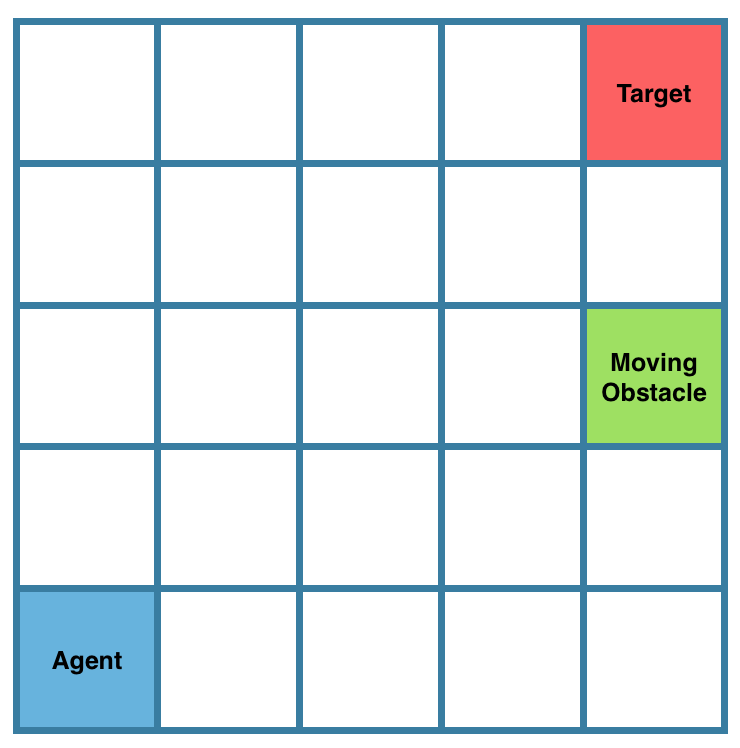
\includegraphics[width=0.23\textwidth]{images/gridworld.png}
  \caption{Simulated social navigation task.} \label{fig:gridworld}
\end{wrapfigure}

% \begin{figure}[t]
%   \centering
%   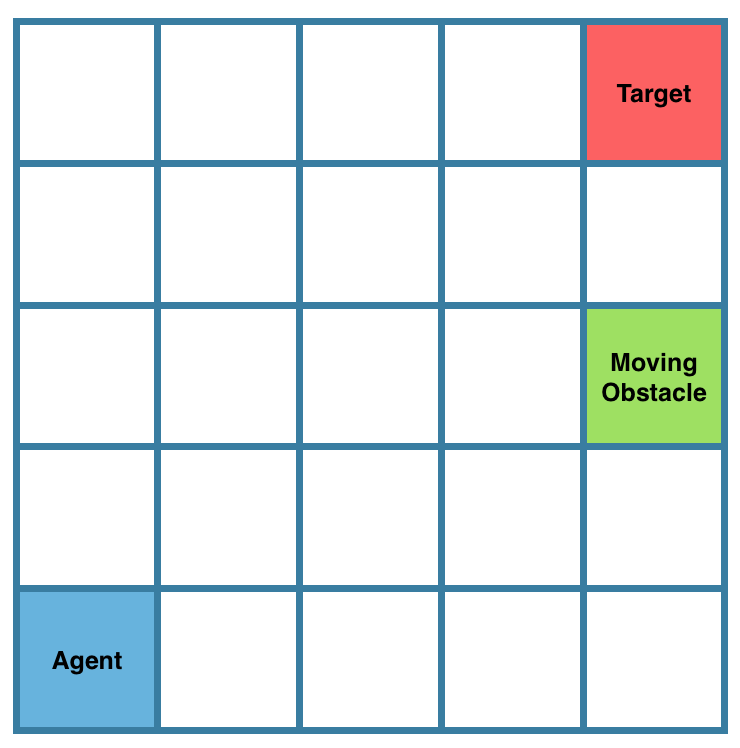
\includegraphics[bb=0 0 533 539,width=0.5\columnwidth]{images/gridworld.png}
%   \caption{Moving obstacle gridworld 	\label{fig:gridworld}}
% \end{figure}
For this domain we first define two ground truth reward functions, $R^{\mathcal{D}^*} = w^{\mathcal{D}^*}\phi(s,a)$, $R^{\mathcal{F}^*} = w^{\mathcal{F}^*}\phi(s,a)$ that represent behaviours we want to learn to immitate and avoid respectively. In our experiments we first sample initial test states, $P^{s_1}_{test}$, which we fix for all experimental runs. These initial conditions along with the policies derived from $R^{\mathcal{D}^*}$, $R^{\mathcal{F}^*}$ produce feature expectations $\widetilde{\mu}^{\mathcal{D}_{test}}$ and $\widetilde{\mu}^{\mathcal{F}_{test}}$ respectively. For each experimental run, we then sample a set of initial train states $P^{s_{1}}_{train}$ and also generate their respective feature expectations $\widetilde{\mu}^{\mathcal{D}_{test}}$,$\widetilde{\mu}^{\mathcal{D}_{train}}$. These feature expectations are used to train reward functions (and subsequently policies) for each of the algorithms considered i.e. IRL, IRLF and the incremental version of IRLF described in algorithm \ref{alg:lff}. Each of these policies, $\pi$ are then paired with $P^{s_{1}}_{test}$, the initial conditions in the test set, to produce the feature expectations for the policy at those initial conditions, $\mu^{\pi^*}|_{test}$. Finally we go on to compute the values of each policy, at those initial conditions, with respect to the two reward functions, $V^{\pi^*}_{\mathcal{D},test} = (w^\mathcal{D})^T\mu^{\pi^*}|_{test}$, $V^{\pi^*}_{\mathcal{F},test} = (w^\mathcal{D})^T\mu^{\pi^*}|_{test}$. $V^{\pi^*}_{\mathcal{D},test}$ should be as high as possible since it measures the value we accumulate based on the reward function we are trying to imitate. $V^{\pi^*}_{\mathcal{F},test}$ on the otherhand should be as low as possible since we $w^{\mathcal{F}^*}$ is a reward function we want to avoid.


% The learner has access to two sets of trajectories, $\mathcal{D}_{train},\mathcal{F}_{train}$, of length $h = 15$. The trajectories in $\mathcal{D}_{train}$ are generated using a reward function $R^\mathcal{D} = w^\mathcal{D}\phi(s,a)$ and summarised by their feature expectations $\widetilde{\mu}^{\mathcal{D}_{train}}$. Likewise the tranjectories in $\mathcal{F}_{train}$ are generated by a reward function $R^\mathcal{F} = w^\mathcal{F}\phi(s,a)$ and summarised by $\widetilde{\mu}^{\mathcal{F}_{train}}$. The underlying ``true'' reward functions $R^\mathcal{D}$ and $R^\mathcal{F}$ represent, respectively, the positive aspects of the domains such as reaching the target, and its negative aspects such as hitting the obstacle. The reward functions are not known to the learner. \jm{need more detail on the reward function. What are the specific numbers for these things? Otherwise, we need to make the code available and link it, for this to be reproducible.}

% Two more sets of trajectories, namely $\mathcal{D}_{test}$ and $ \mathcal{F}_{test}$, are used to assess the learner's performance on the task. The evaluation takes place by measuring the value accumulated by the agent based on the respective dataset's true reward function. Using equation \eqref{eq:parametrized_value} this is simply,
% \begin{align}
% &V^{\pi}_{\mathcal{D}} = (w^\mathcal{D})^T\mu^\pi|_\mathcal{D}\\
% &V^{\pi}_{\mathcal{F}} = (w^\mathcal{F})^T\mu^\pi|_\mathcal{F}. \label{eq:value_on_expert}
% \end{align}
% In other words, we can use the weights for each of the reward functions, along with the feature expectations associated with the execution of a policy from a certain set of initial conditions, to measure the performance of the agent with respect to that reward function. If therefore follows that a well-performing algorithm will maximise $V^{\pi}_{\mathcal{D}_{test}}$ and minimise $V^{\pi}_{\mathcal{F}_{test}}$. 

% In our experiments we fix $10$ test states (and their respective feature expectations) and perform experimental runs, for which we train our IRLF algorithm and its original counterpart, the MaxCausEnt IRL algorithm, on randomised initial conditions. The performance of the learned reward functions (and policies) at the fixed initial test states is evaluated using \eqref{eq:value_on_expert}. \jm{this sentence doesnt make sense.}\ks{I wanted to say that we learn on some initial conditons and test on others.}

We compare the performance of the two algorithms on two scenarios within this simulated domain. In the first scenario, the true weights $w^{\mathcal{D}^*}$ reward reaching the target and avoiding the obstacle, while $w^{\mathcal{F}^*}$ gives a large reward to being in the same cell as the obstacle. We call this the \emph{constrastive} scenario. In the second, or \emph{complementary} scenario, $w^{\mathcal{F}^*}$ is as before, but now $w^{\mathcal{D}^*}$ only rewards reaching the target. The constrastive scenario aims to investigate whether there are any benefits to learning from failure when the successful dataset already shows the complete desired behavior, but the failed demonstrations provide additional information regarding undesired behavior. The complementary scenario investigates whether we can learn part of the desired behavior from $w^{\mathcal{D}^*}$ (reaching a target), and part of it from $w^{\mathcal{F}^*}$ (avoiding the obstacle). 

Figure \ref{fig:toy_expert_apprentice_contrastive} demonstrates the performance of IRLF (blue,green) and Maximum Causal Entropy IRL (red), on the constrastive scenario when evaluated on $w^{D}$. We can see that our algorithms
converge to a value that is higher than that of their original counterpart. This is a first indication that IRLF successfully utilises failed demonstrations to learn better and faster. Very interesting results can also be observed in Figure \ref{fig:complementary} for the complementary scenario. It should be apparent that IRLF not only it achieves the same value as the test data in \ref{fig:toy_expert_apprentice_complementary} but also manages to accumulate less value than even the successful test data, in \ref{fig:toy_taboo_apprentice_complementary}, when evaluated on the reward function for the failed demonstrations (black). This clearly indicates that the learner is imitating the successful demonstrations while keeping away from the failed demonstrations. Note finally the predicted oscilatory behaviour that results from updating $w^\mathcal{F}$ directly.

% Our first set of experiments consider a moving obstacle Gridworld domain, shown in figure \ref{fig:gridworld}.
% In this domain an agent moves in an environment, containing a moving obstacle, that could be moving either vertically
% or horizontally and a target that is stationary. The goal of the agent is to reach the target, while avoiding 
% the obstacle. The learning agent or \emph{apprentice} is not familiar with the task, yet he is provided with some data coming from two other agents
% each with different aims. The first of these agents is an \emph{expert} at the task, his reward function ($R_e = \theta_e\phi(s,a)$) is large and negative
% for being in the same cell as the obstacle, and it is large an positive for reaching the target. The second agent is a
% \emph{taboo} agent with a reward function $(R_t=\theta_t\phi(s,a))$ that is positive for colliding with the obstacle. Since we know the reward functions used for learning, we can directly evaluate the properties of our method. 

% Our experiments in this domain involve choosing five random initial train and test states for our agents $b_{0_{test}}$,$b_{0_{train}}$ and generating data for 15 decision steps. We then use the data generated using $b_{0_{train}}$ to train the apprentice, resulting in a learned reward function, $R_a = \theta_a\phi(s,a)$ and the apprentice policy $\pi(s,a)_a$. Using this policy we perform trajectories using the initial conditions in $b_{0_{test}}$. These trajectories produce feature expectations for the model, which when multiplied with either of the weight vectors $\theta_e,\theta_t$ will \sw{present tense} give us the accumulated value for those initial states based on the reward functions of either the expert or the taboo. In other words if the apprentice generates feature expectations $\Phi_{\pi(s,a)_a}$ the Value \sw{WHY?} of the apprentice based on the expert reward function is simply $\theta_e^T\Phi_{\pi(s,a)_a}$ \jm{wait, so with our method this value is $0$? c.f. Table 1}. In addition to the difference in value, we also measure the absolute difference of the learned policies between apprentice and expert $(\pi(s,a)_e - \pi(s,a)_a)$. 
% \jm{How are you calculating differences between policies? KLD?} We repeat this procedure 20 times with different initial train and test conditions, and report the results in Table \ref{tab:results} \sw{?} , an example run is shown in figure \ref{fig:results} \sw{unpunctuated run-on sentence.}

\begin{figure*}[t]
  \centering
  \begin{subfigure}[b]{0.475\columnwidth}
    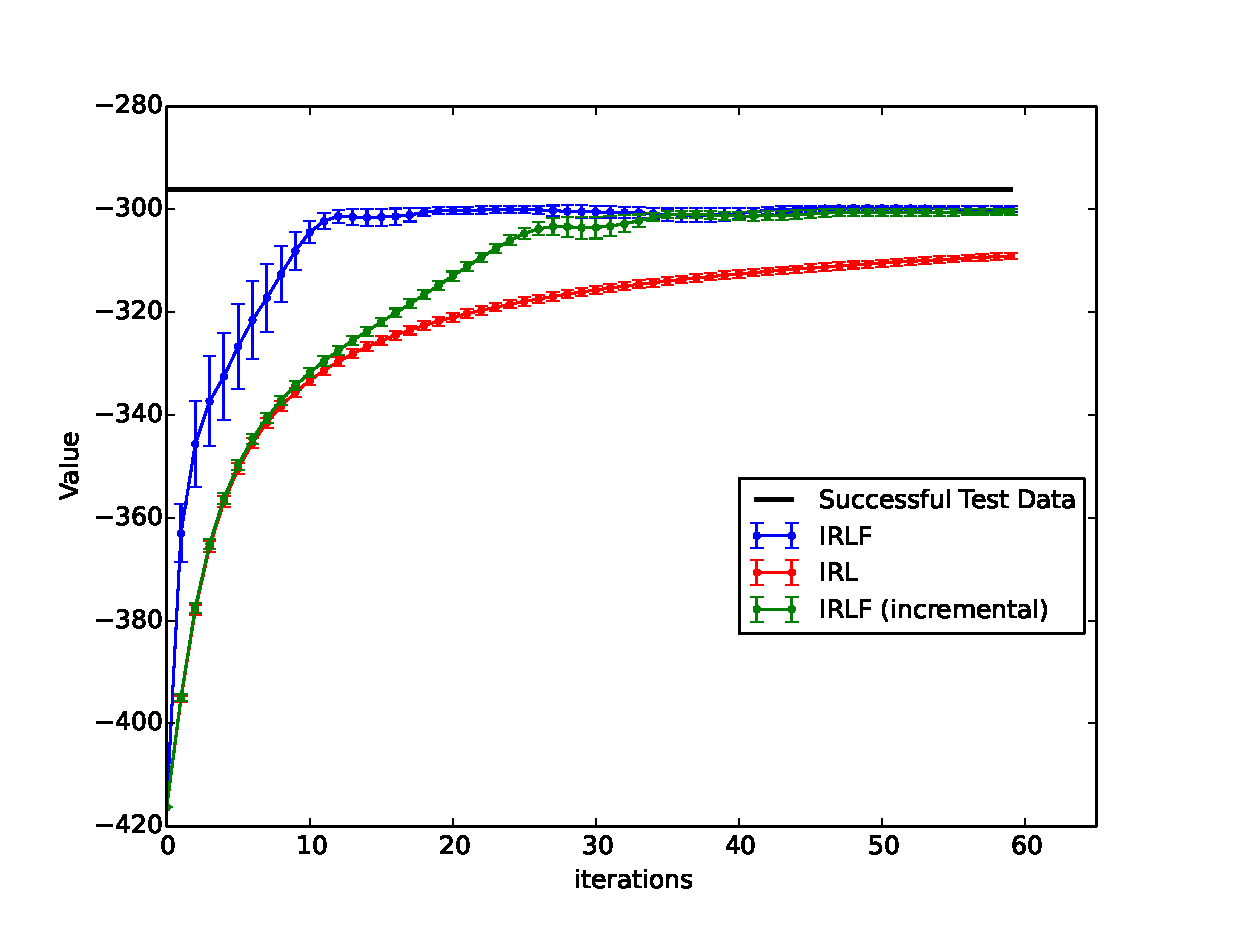
\includegraphics[trim=0.5cm 1cm 2cm 0,clip=true,width=\textwidth]{images/expert_apprentice_contrastive.eps}
    
    \caption{Contrasting w.r.t.\ $w^\mathcal{D}$}
    \label{fig:toy_expert_apprentice_contrastive}
  \end{subfigure}
  \hfill
  \begin{subfigure}[b]{0.475\columnwidth}
    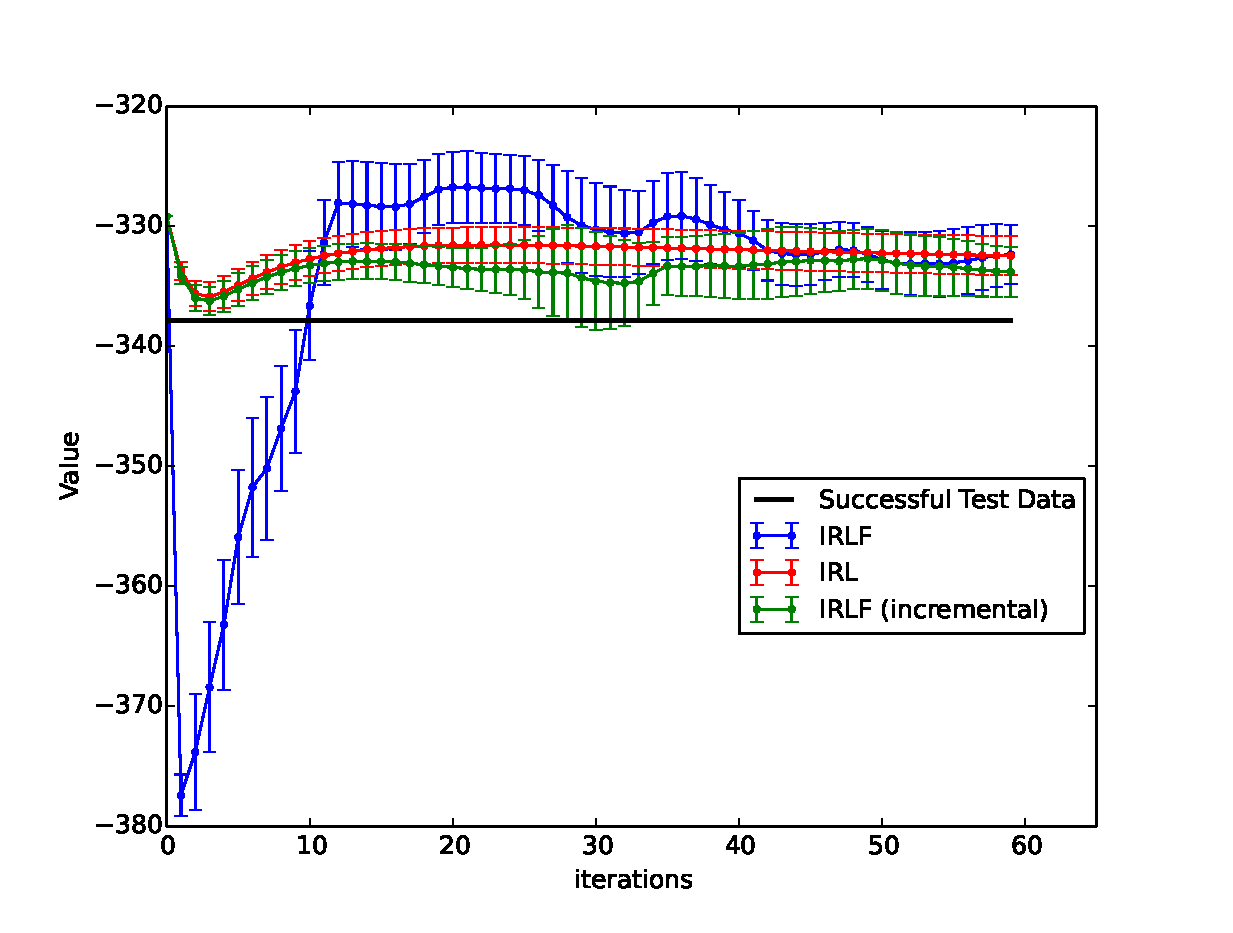
\includegraphics[trim=0.5cm 1cm 2cm 0,clip=true,width=\textwidth]{images/taboo_apprentice_contrastive.eps}
    
    \caption{Contrasting w.r.t.\ $w^\mathcal{F}$}
    \label{fig:toy_taboo_apprentice_contrastive}
  \end{subfigure}  
  \label{fig:contrastive}
  \begin{subfigure}[b]{0.475\columnwidth}
    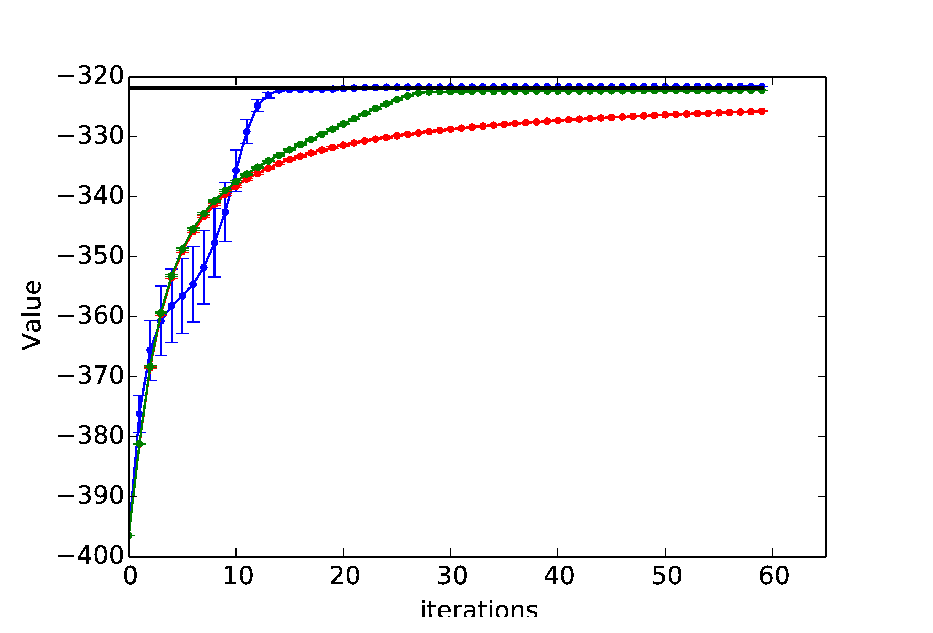
\includegraphics[trim=0.5cm 1cm 2cm 0,clip=true,width=\textwidth]{images/expert_apprentice_complementary.eps}
    
    \caption{Complementary w.r.t.\ $w^\mathcal{D}$}
    \label{fig:toy_expert_apprentice_complementary}
  \end{subfigure}
  \hfill
  \begin{subfigure}[b]{0.475\columnwidth}
    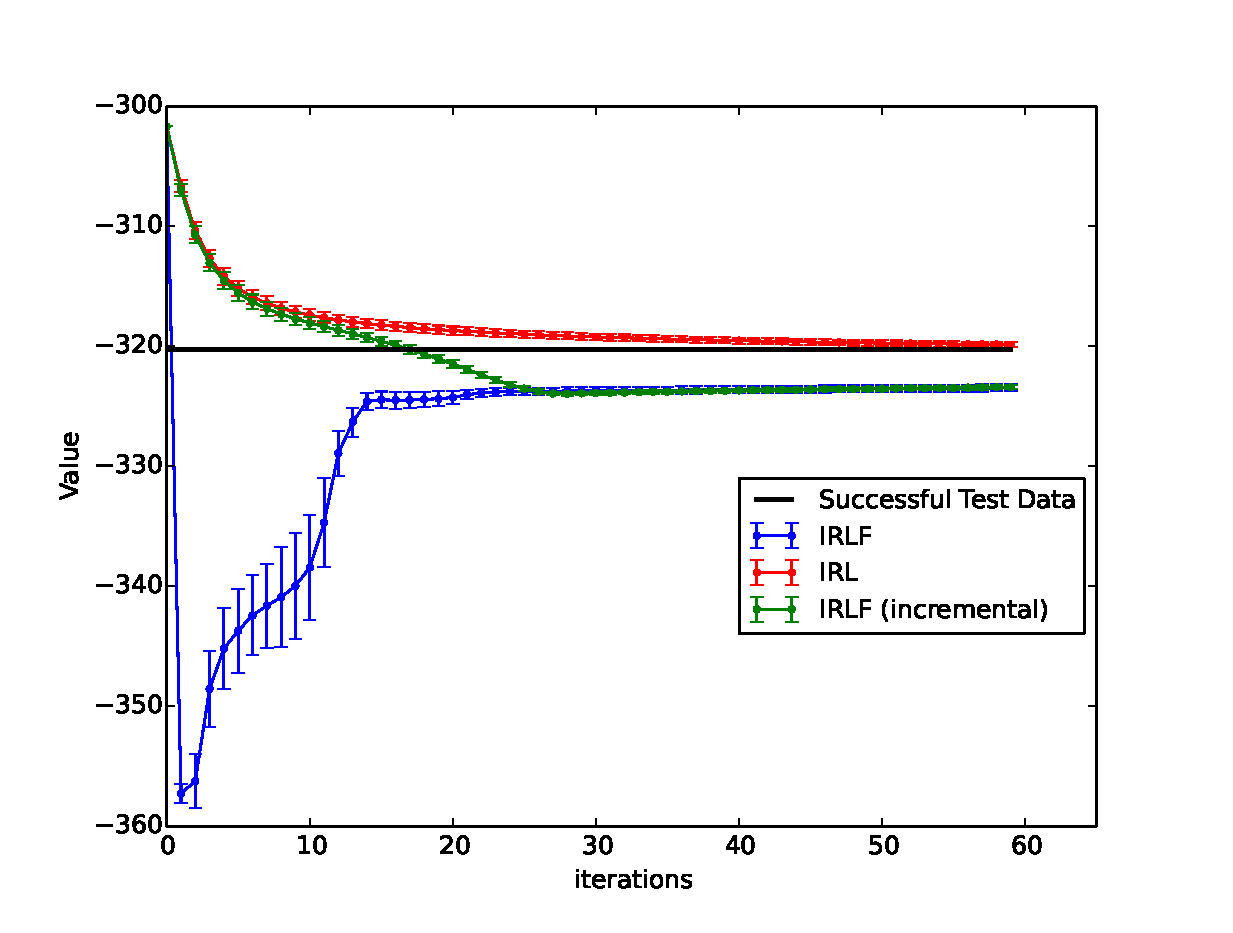
\includegraphics[trim=0.5cm 1cm 2cm 0,clip=true,width=\textwidth]{images/taboo_apprentice_complementary.eps}
    \caption{Complementary w.r.t.\ $w^\mathcal{F}$}
    \label{fig:toy_taboo_apprentice_complementary}
  \end{subfigure}  
  \caption{Value in constrasting and complementary simulated domains w.r.t.\ $w^\mathcal{D}$ and $w^\mathcal{F}$. }
  \label{fig:complementary}
\end{figure*}

% \begin{table}[]
% \centering

% \label{tab:results}
% \begin{tabular}{|l|l|l|l|}
% \hline
%            & $\theta_e(\Phi_{a}-\Phi_{e)}$& $\theta_t(\Phi_{a}-\Phi_{t)}$ & $|\pi_a - \pi_t|$ (\%) \\ \hline
% Original   & -6.125(2.06)        & 2.41(1.82)         & 15                    \\ \hline
% Our Method & 0(0.2)              & 0.02(0.167)        & 10                    \\ \hline
% \end{tabular}
% \caption{Results on test set after 20 runs of random initial conditions. $\theta_e$ represent reward weights, $\pi$ represents policy and $\Phi$ represents feature expectations. The subscripts $a,e,t$ represent the apprentice, expert and taboo agents respectively. \jm{This table needs to be cleaned up. Try to keep the same number of significant figures in all entries.}}
% \end{table}
% REAL DATA SECTION %
\subsection{IRLF on real data}
Taking into account the encouraging performance of IRLF on a relatively simple domain, we now go on to investigate its capabilities in a much more complicated task. We consider real data
of social robot navigation within a room of dimentions 5mx5m, with a target and a moving (or standing) person \ks{figure here?}. The successful dataset $\mathcal{D}$, is collected by an expert driving the robot towards the target while avoiding the obstacle in a socially appropriate way. The failed dataset $\mathcal{F}$ is collected by driving the robot in a simulator. After collecting the two required datasets, we need to model the problem as an MDP. The state space $S$, in this case consists of discretised positions for both the obstacle and the robot, as well as the discretised orientation of the obstacle, yielding a total of 809,500 states. The action space $A$ consists of 8 robot orientations, and an action that accounts for the robot being stopped. Using this definition of state-action space we proceed to calculate a factored stochastic transition function $\mathcal{T}$ that dictates the world dynamics. Finally, our feature set $\phi(s,a)$ consists of 1401 binary features, encoding the relative position of the robot from both the target and the obstacle, as well as their relative orientations. \\
\ks{Missing a link here}
Unfortunatelly, this time we have no ground truth reward function that would allow us to compute the value accumulated by the learner, as we did in the previous section. On artificial domains like the ones presented in \cite{levine2011nonlinear}, the knowledge of the reward function allows for precise evaluation of an algorithm's performance on the task. But in all work where real data is involved researchers either consider visual demonstrations of results as in \cite{ratliff2006maximum}, or domain specific performance measures as in \cite{neu2009training}. In terms of social navigation \cite{vasquez2014inverse} use hand designed evaluation to compare and select feature sets and algorithms. In our case it seems like none of the above evaluation measures is sufficient to demonstrate the strengths of IRLF, so we resort to an intermediate solution. We run MaxEnt IRL -though any other algorithm can be used at this point- on the collected datasets $\mathcal{D}$ and $\mathcal{F}$ and derive reward functions, $R^{\mathcal{D}}$ and $R^{\mathcal{F}}$. This brings us to a similar situation as in the previous section, with the very important difference that the reward functions we will be generating data from, are no longer handcoded but derived from \emph{real} data. Figure \ref{fig:paths} demonstrates trajectories generated from the two reward functions. We can see that $R^{\mathcal{D}}$ produces feasible, human-like trajectories, while $R^{\mathcal{F}}$ generates very inapropriate behaviour for a robot.\\
\vspace{-0.3mm}
Our experiments proceed in exactly the same manner as in the toy domain. We generate training trajectories from our reward functions and use them as inputs to our IRL algorithms whose performance is then evaluated using a separate set of test trajectories. The results for 20 runs of our experiments are shown in figure REF. Our first observation is that the incremental version of IRLF is clearly superior to the original MaxCausEnt algorithm, with behaviour that is very similar to that in the toy domain. This consistency supports the two main arguements of our work. Data of failed demonstrations is a useful tool for IRL allowing it to generalise better to new unseen conditions, and IRLF is an effective tool for leveraging this data thereby extracting the useful information it contains.

\begin{figure}[t]
  \hspace{-10pt}
  \begin{subfigure}{0.22\textwidth}
    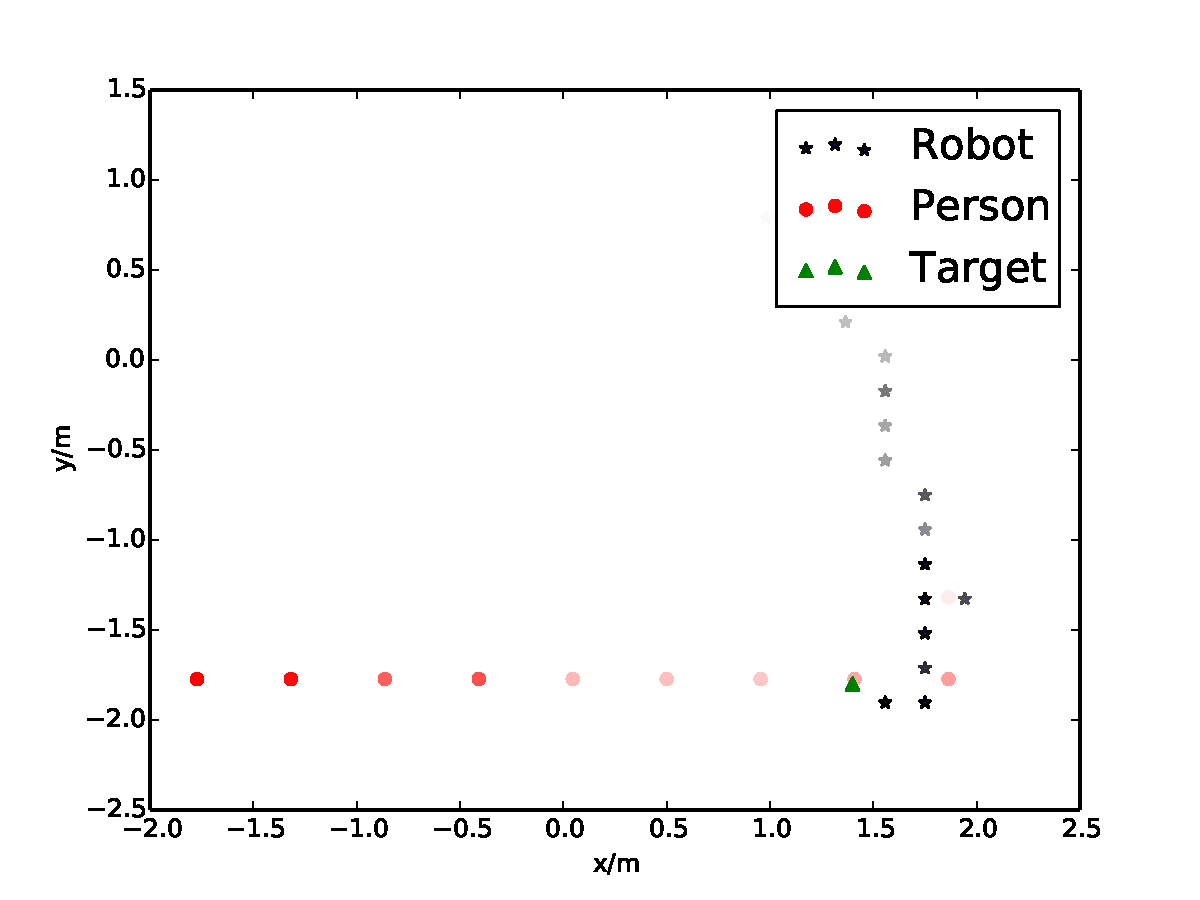
\includegraphics[scale = 0.24]{images/good_path.pdf}
    \label{fig:good_path}
  \end{subfigure}
  \hspace{15pt}
  \begin{subfigure}{0.22\textwidth}
    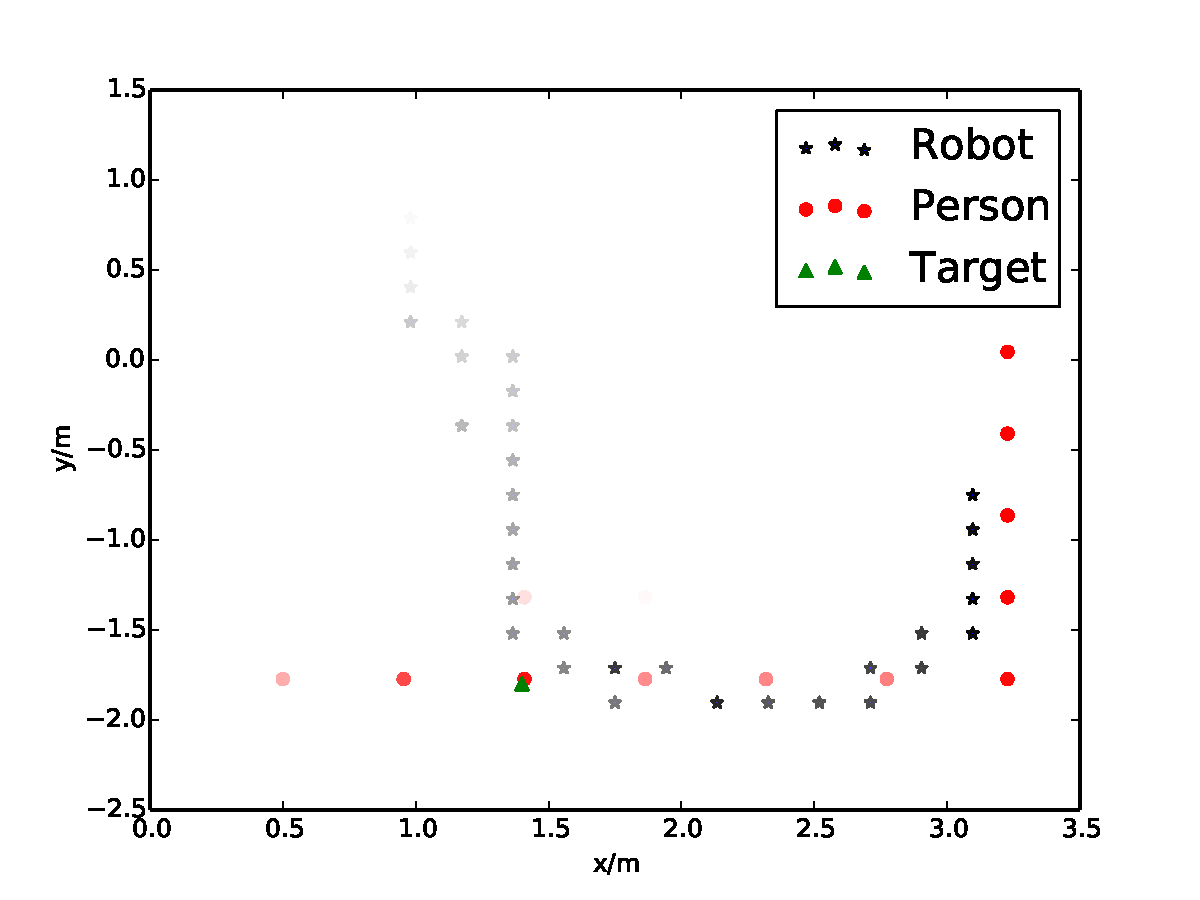
\includegraphics[scale = 0.24]{images/bad_path.pdf}
    \label{fig:bad_path}
\end{subfigure}
  \caption{\small{Sample trajectories from $R^\mathcal{D}$(left) and $R^\mathcal{F}$ (right). These reward functions were learned from real data. The alpha channel denotes time}}
  \label{fig:paths}
\vspace{-4mm}
\end{figure}
\section{Conclusions and Future Work}

\sw{This can be modeled on the new abstract once it's written.  We do need some future work ideas.} \jm{Perhaps we can mention further robot tests and validation of these results as future work. There was also this idea on the table of coupling this learning from failure approach with other IRL / LfD algorithms}

In this paper we have introduced a new framework for Inverse Reinforcement Learning that allows an agent to not only imitate certain behaviours but to also avoid others. The benefits this approach is that it allows otherwise useless data to be used and further enables a designer to inject prior information in the learning, by specifying, through simulated data, what behaviours should be avoided. We have derived a theoretically sound method by directly modifying the derivation of the Maximum Entropy and carrying that through to MaxEnt IRL, providing solutions to the computational obstacles that arise. We have further performed exhaustive experiments in a toy domain, that clearly demonstrate that our method can generalise much better that the baseline IRL algorithm. Finally we have performed learning on real data, again showing that our method is superior to the baseline.  

\sw{There are very few refs.  Can't we think of any more relevant stuff to cite?}

\bibliographystyle{aaai}
\bibliography{references}
	
\end{document}
